\subsection{Unsicherheitsrechnung}\label{VGuD}

\begin{figure}[h]
	\begin{equation*}
		x = \sum_{i=1}^{N} x_i
		;\quad
		u(x) = \sqrt{\sum_{i = 1}^{N} u(x_i)^2}
	\end{equation*}
	\caption{Formel für kombinierte Unsicherheiten des selben Typs nach GUM.}
	\label{fig:GUM_combine}
\end{figure}

\begin{figure}[h]
	\begin{equation*}
		f = f(x_1, \dots , x_N)
		;\quad
		u(f) = \sqrt{\sum_{i = 1}^{N}\left(\pdv{f}{x_i} u(x_i)\right) ^2}
	\end{equation*}
	\caption{Formel für sich fortpflanzende Unsicherheiten nach GUM.}
	\label{fig:GUM_formula}
\end{figure}

\subsection{Oszilloskopkurven}

\begin{figure}[ht]
	\centering
	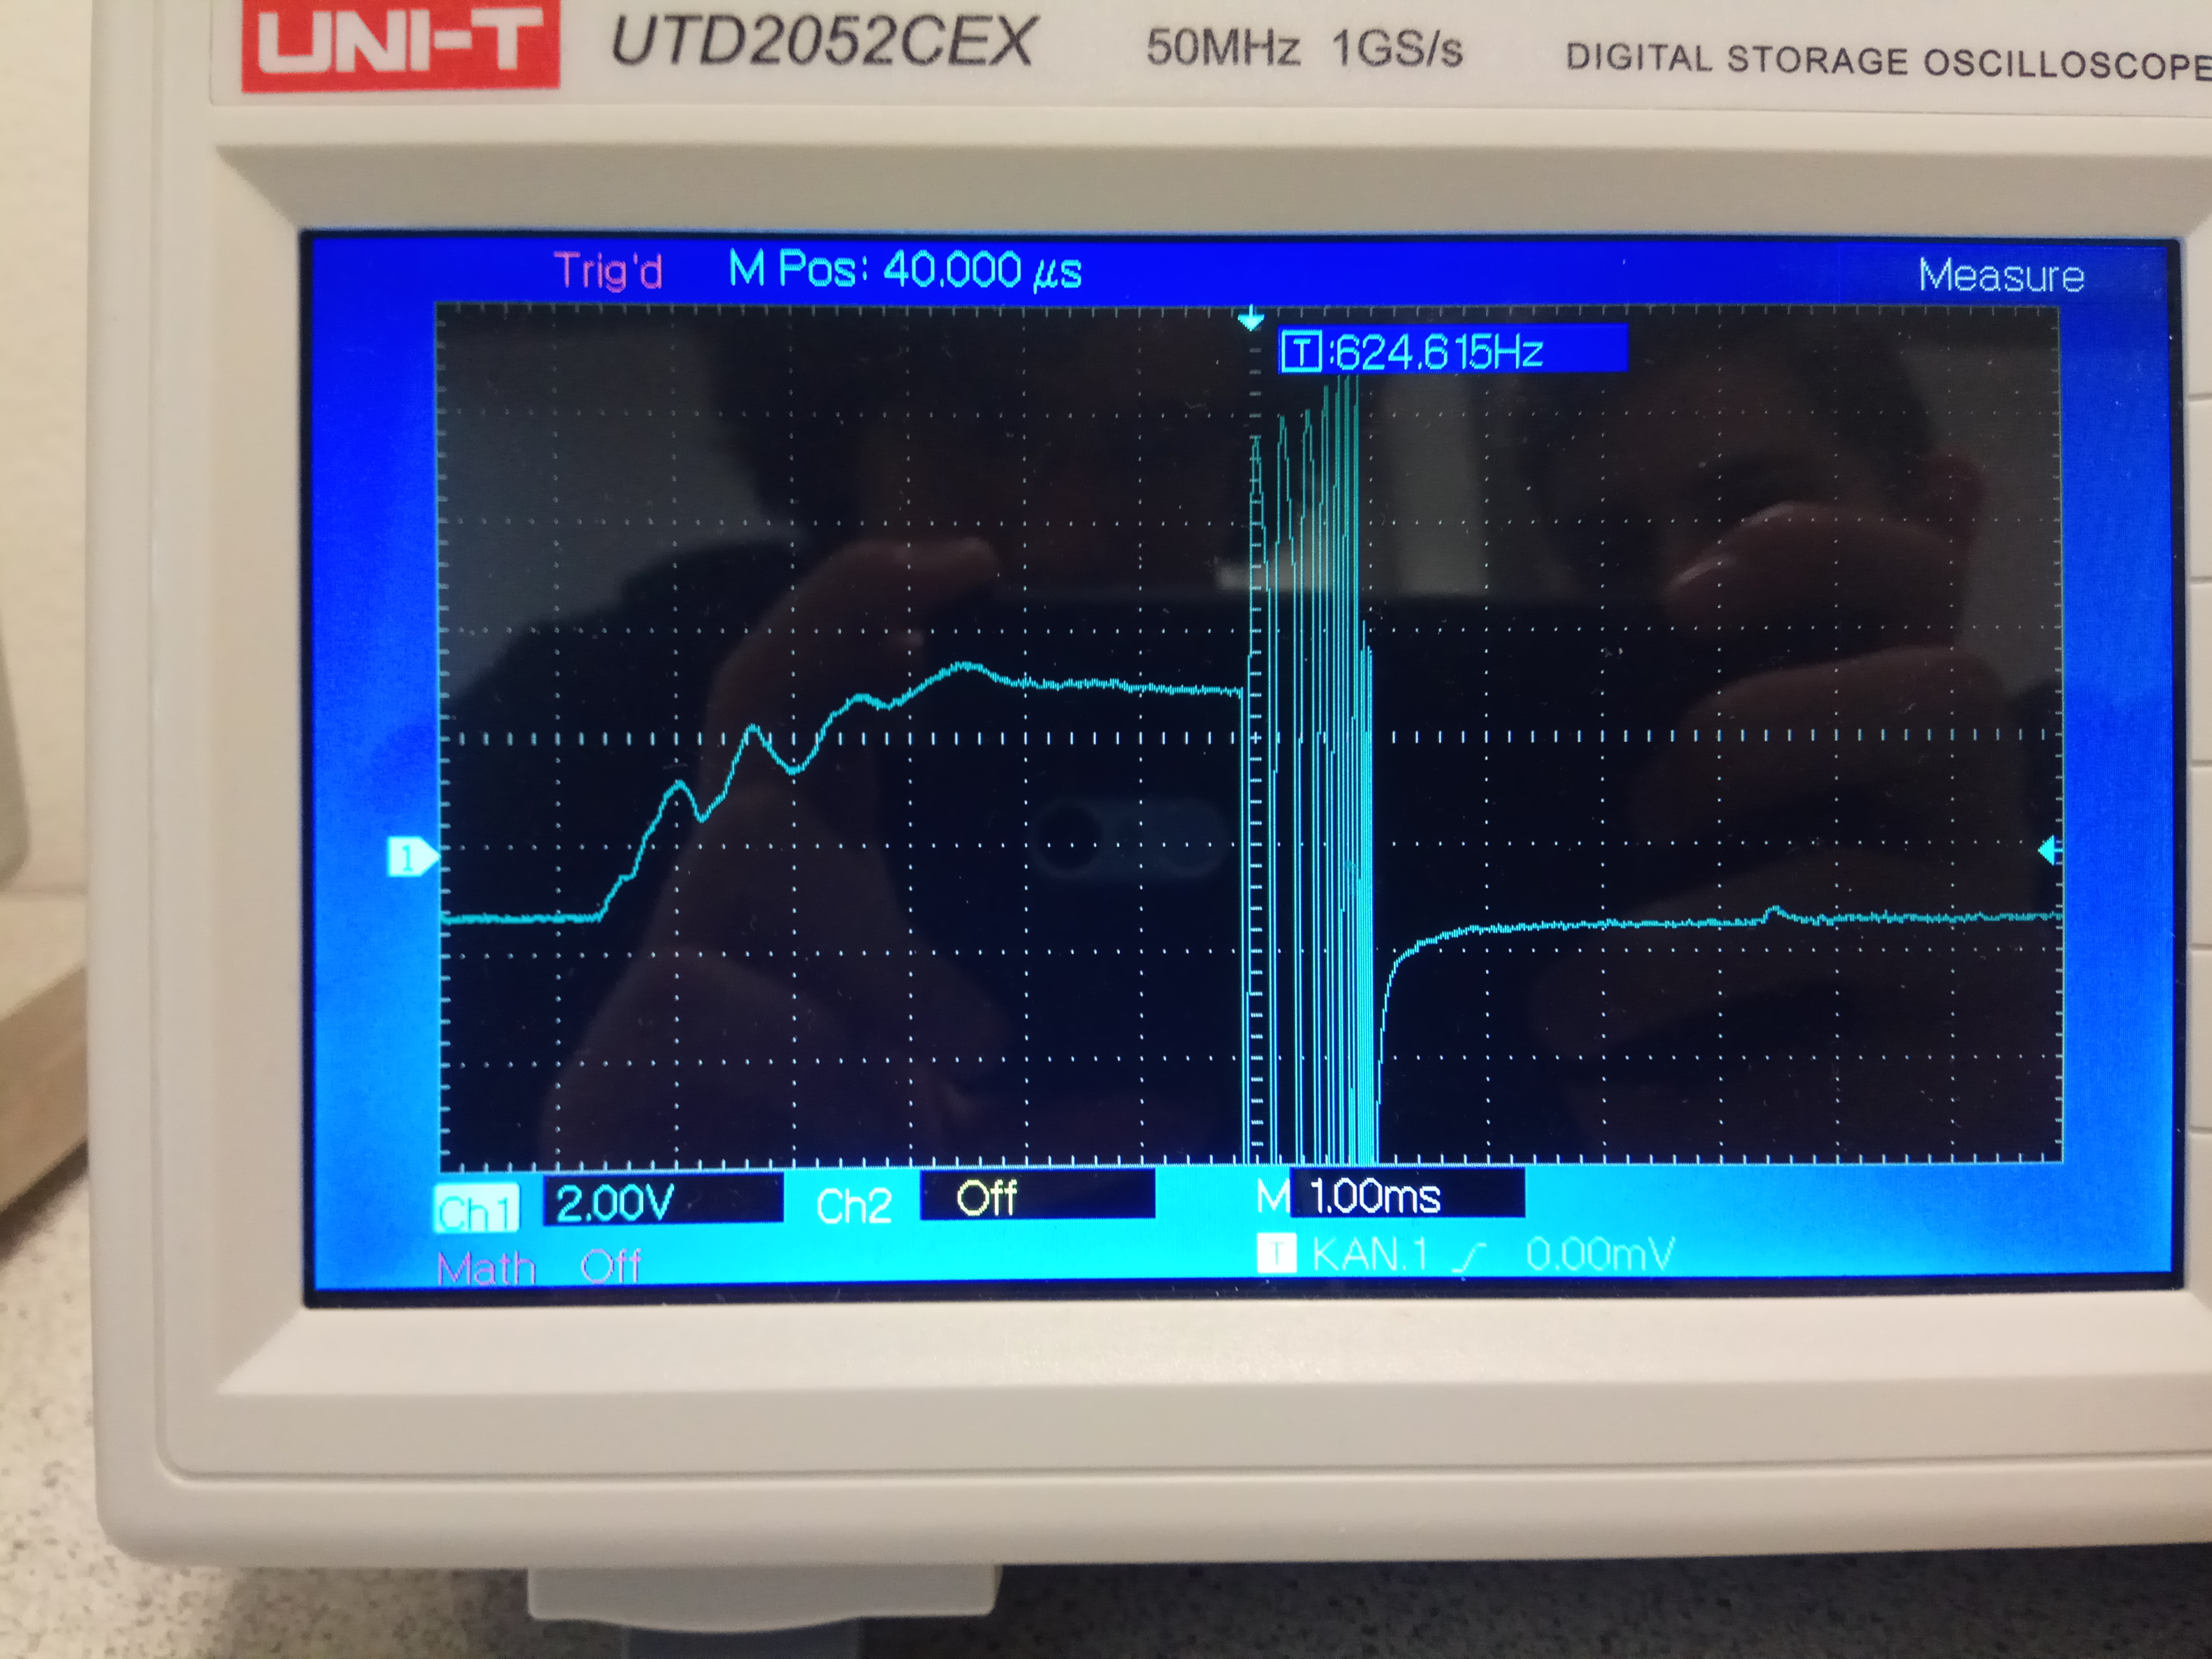
\includegraphics[width=0.8\textwidth]{bilder/ne.jpg}
	\caption{Franck-Hertz-Kurve des Neons am Oszilloskop. Das Relikt in der Mitte ist zu vernachlässigen.}
	\label{fig:kurveNe}	
\end{figure}

\begin{figure}[ht]
	\centering
	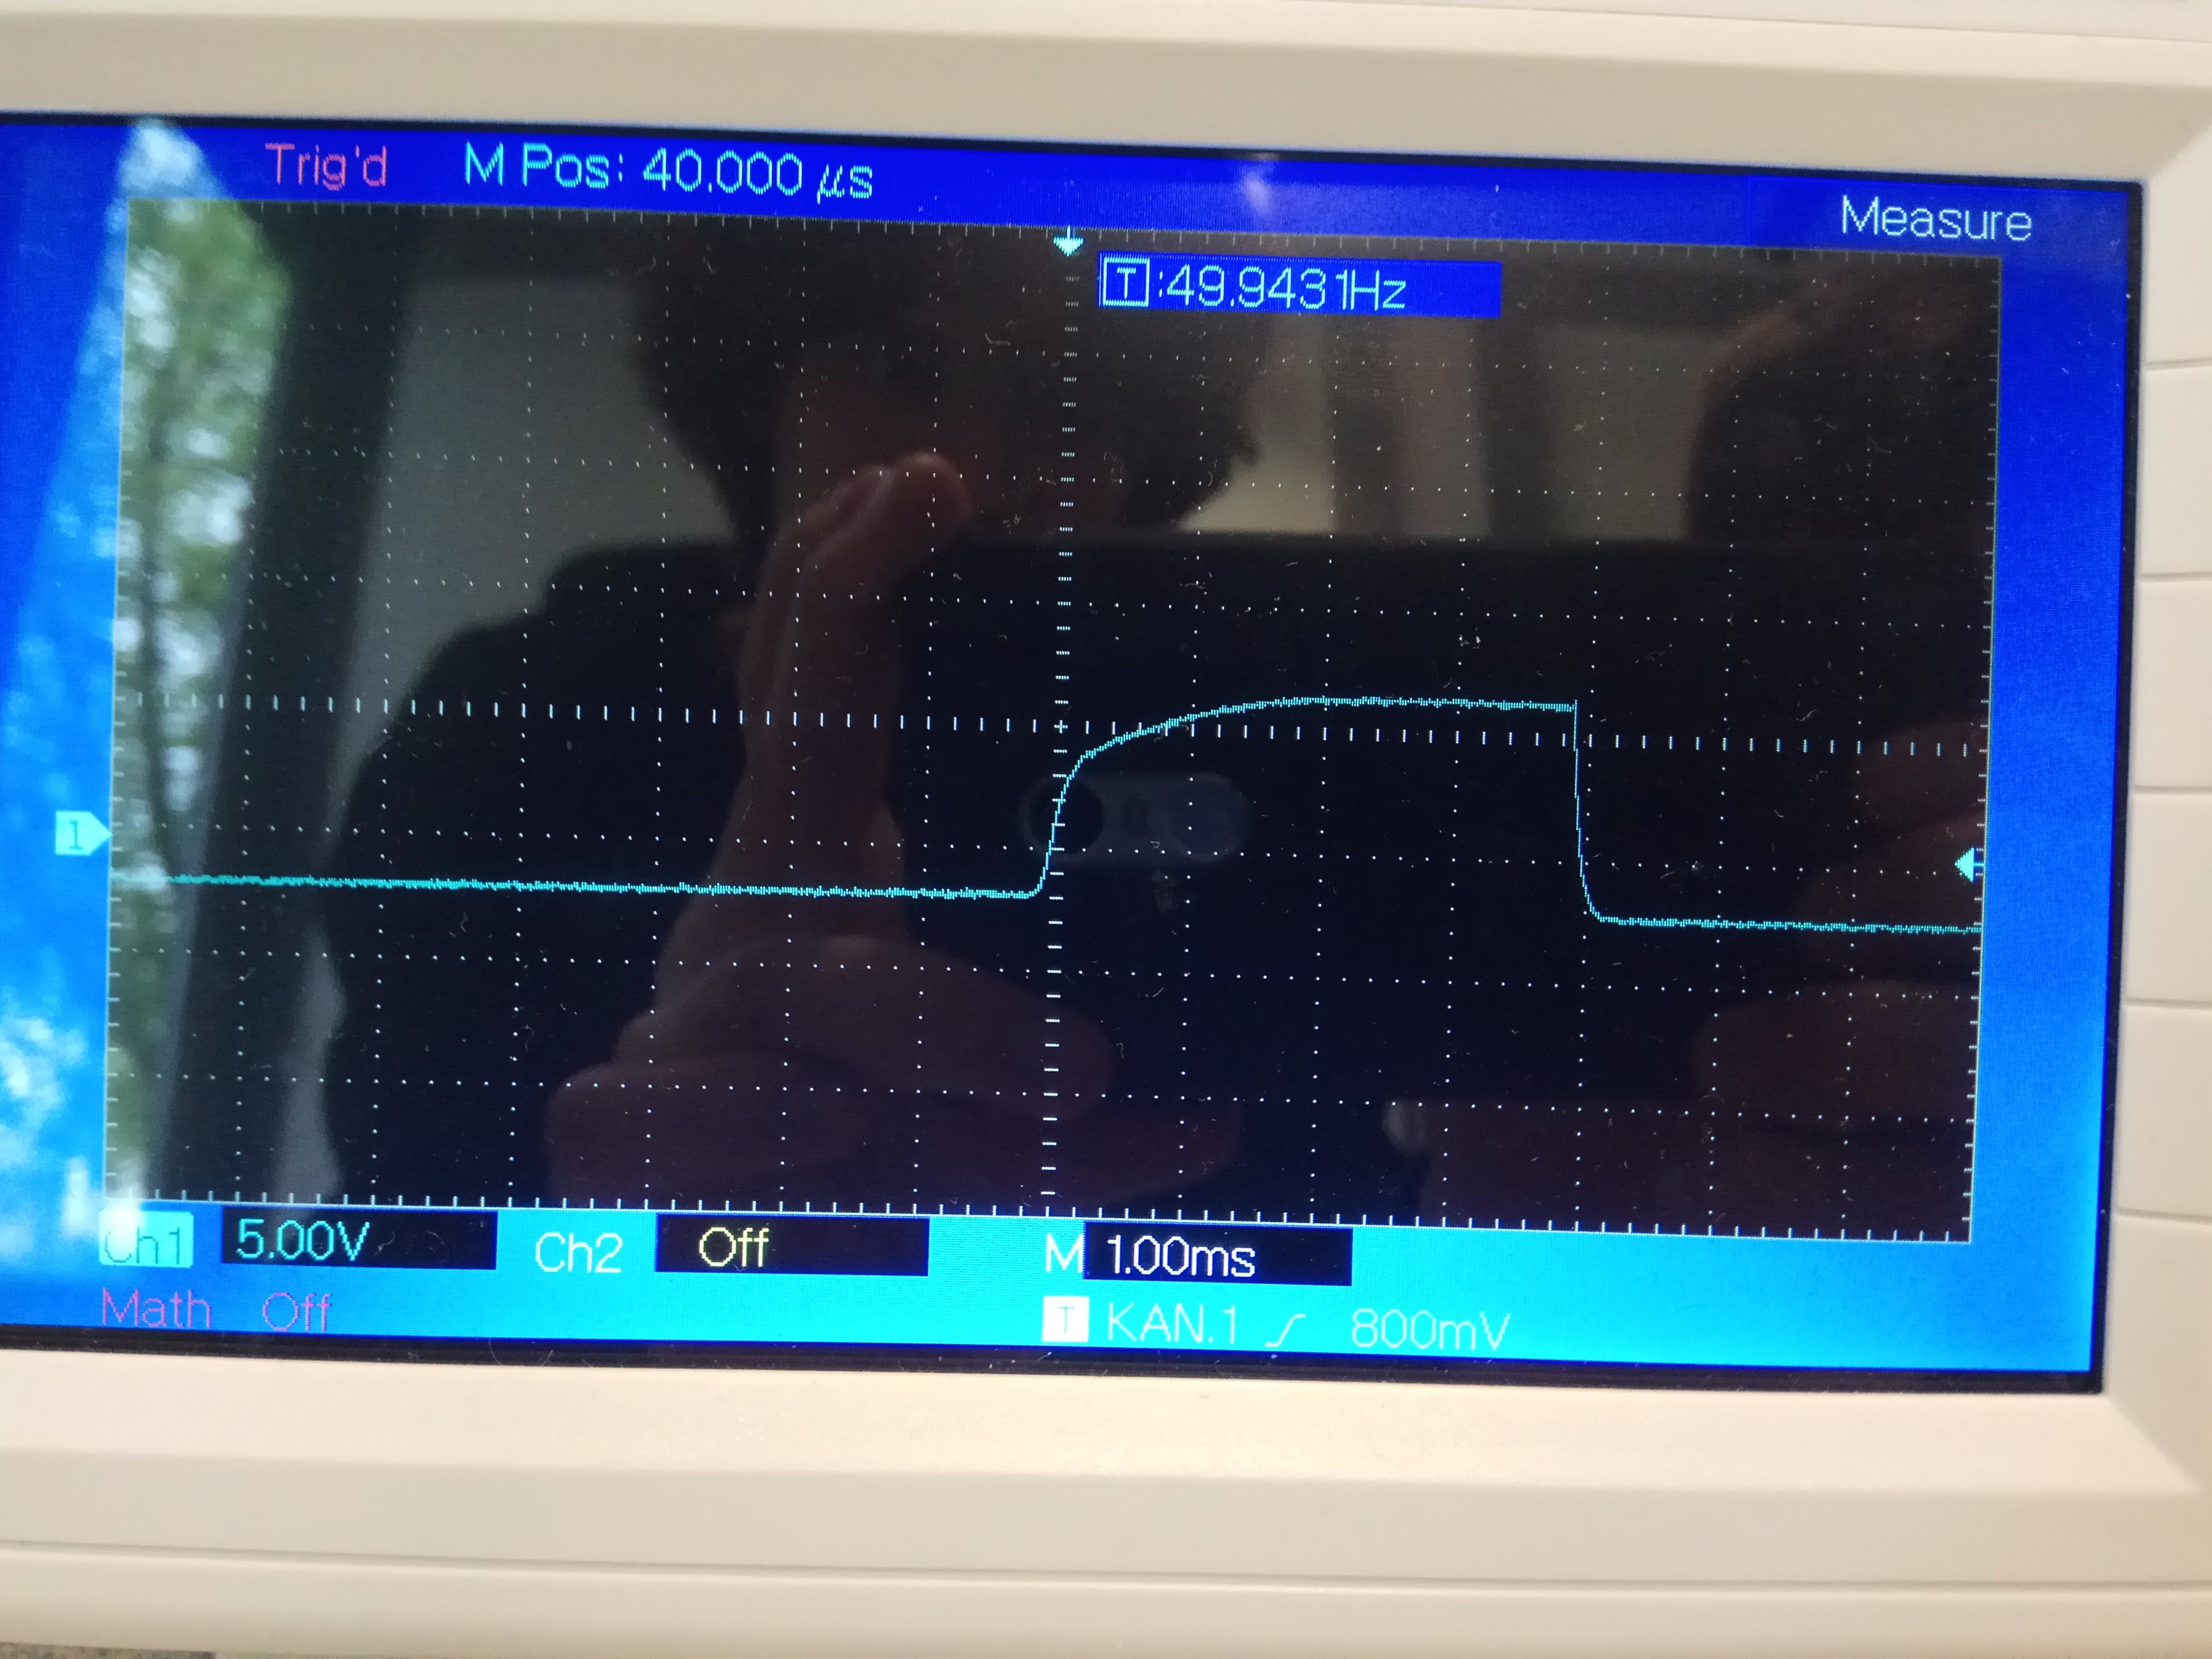
\includegraphics[width=0.8\textwidth]{bilder/hgl.jpg}
	\caption{Franck-Hertz-Kurve des Quecksilbers bei Raumtemperatur am Oszilloskop.}
	\label{fig:kurveHgl}	
\end{figure}

\begin{figure}[ht]
	\centering
	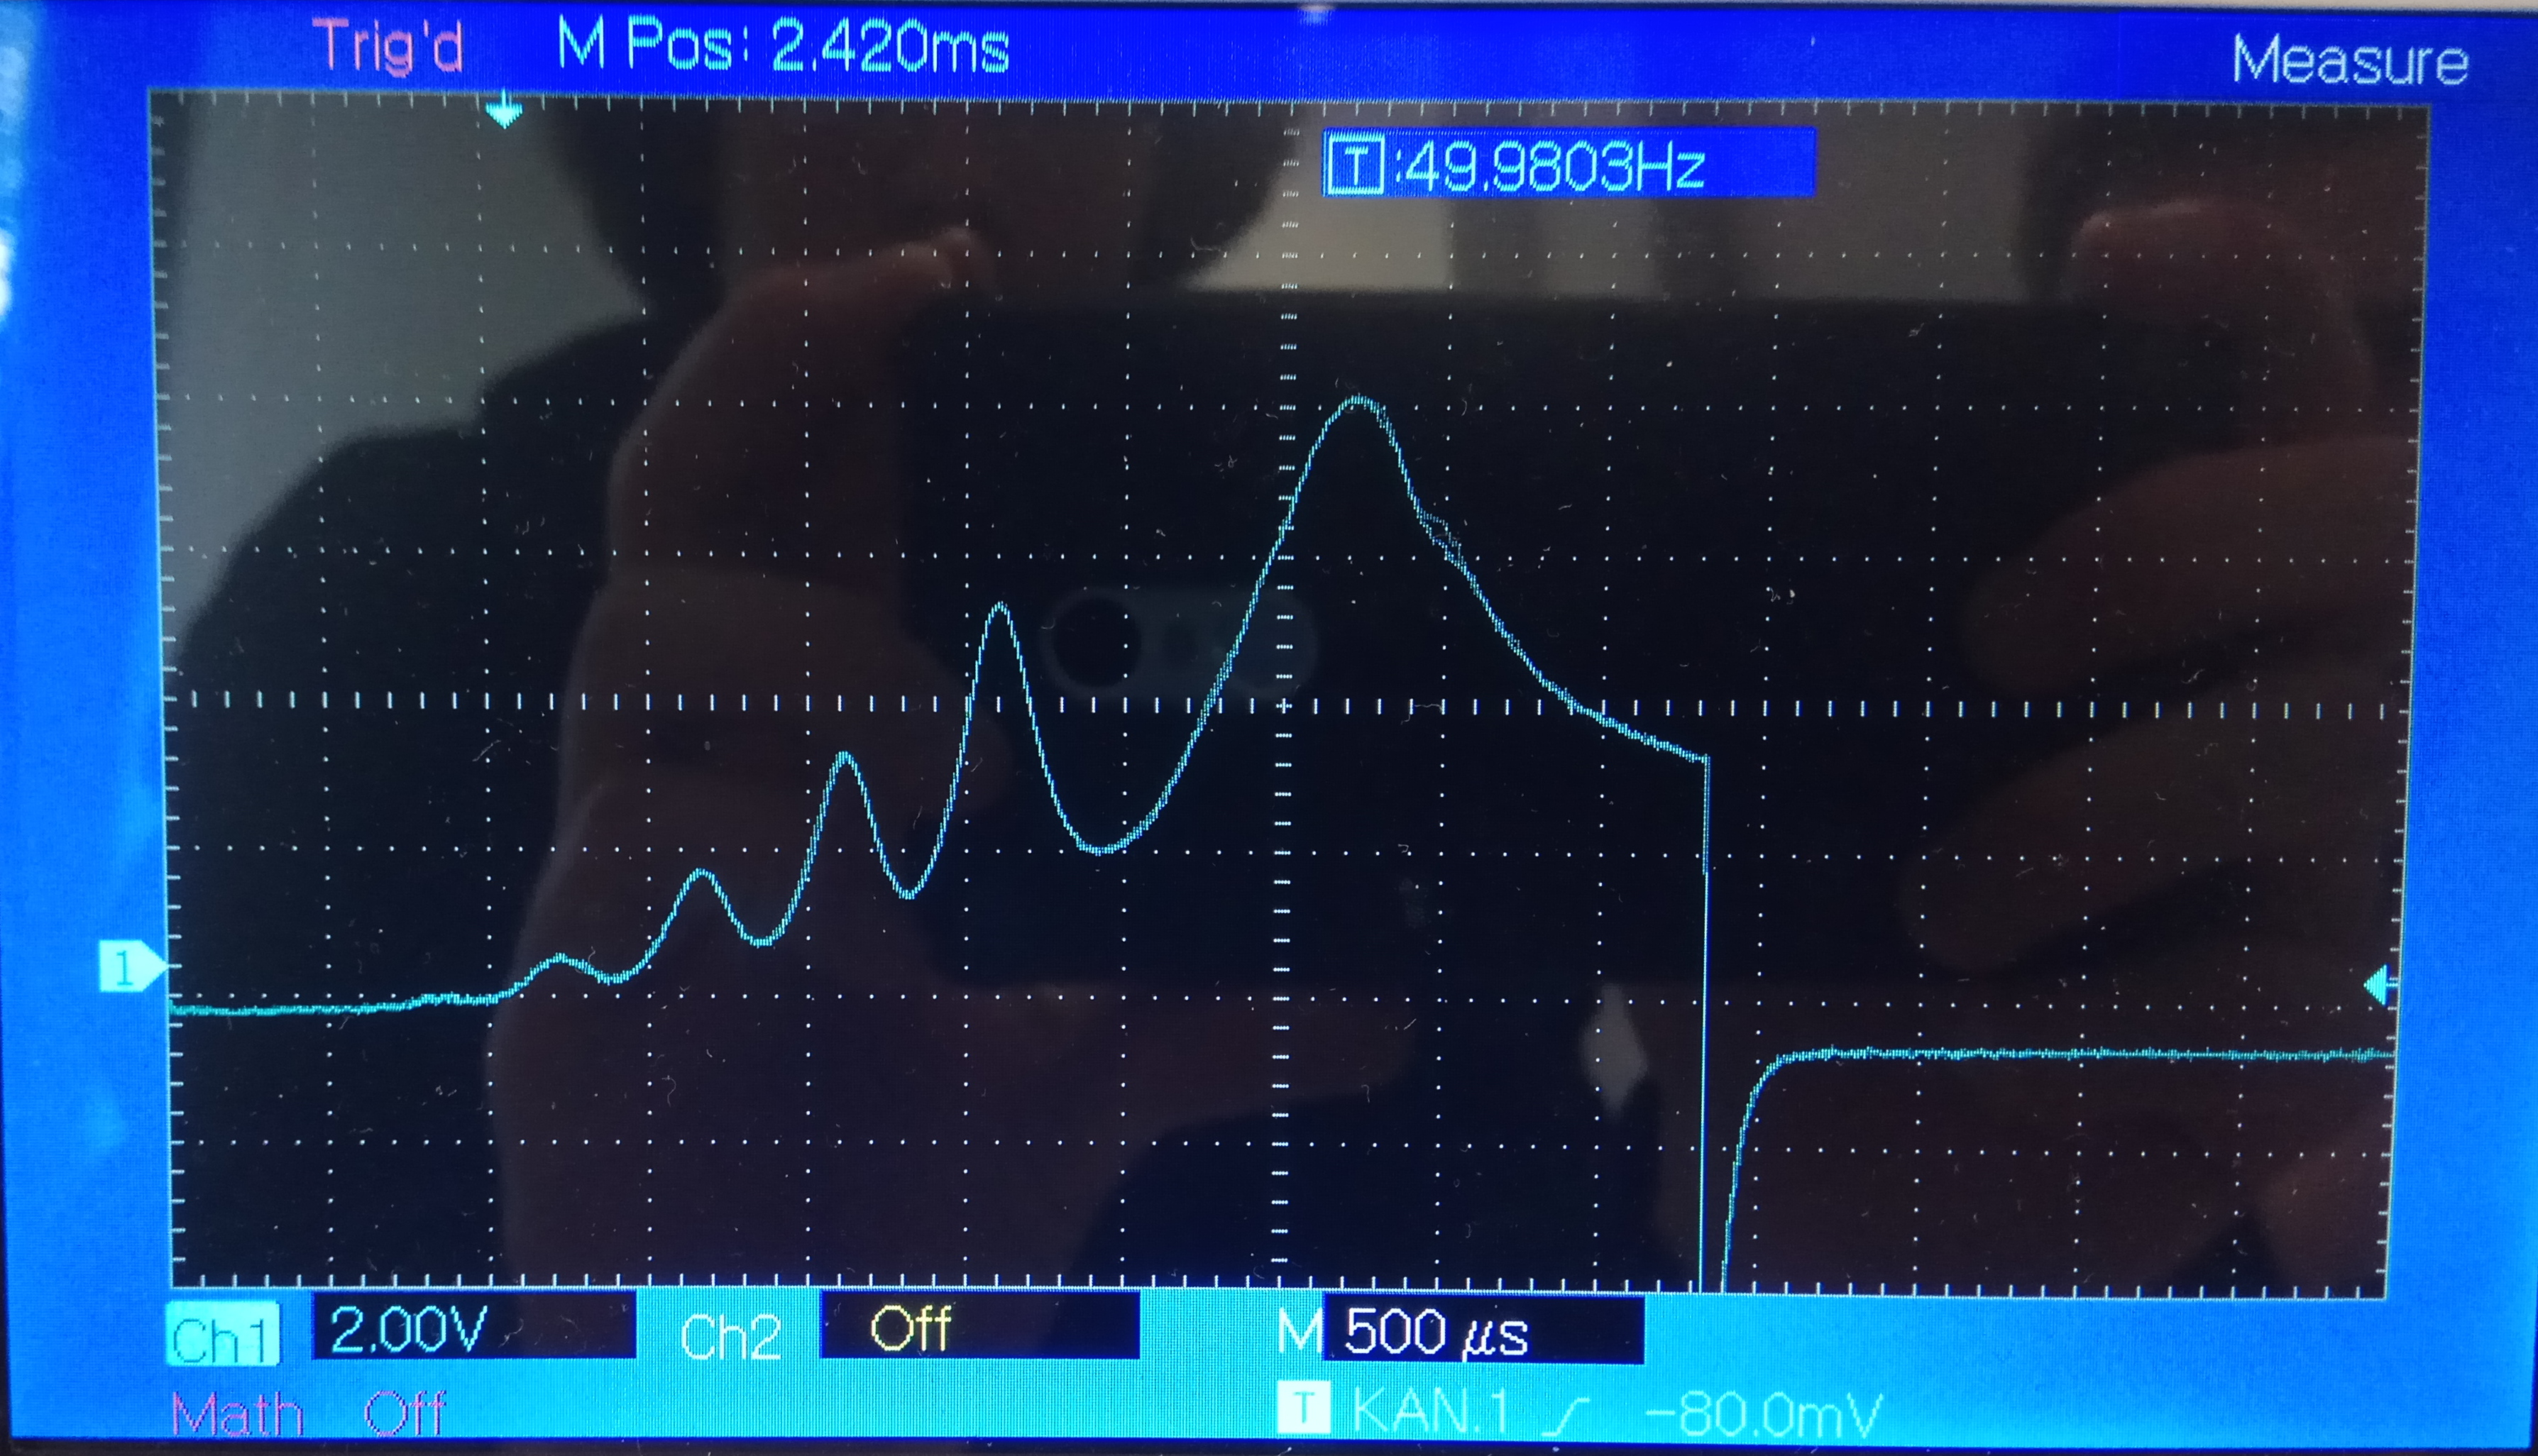
\includegraphics[width=0.8\textwidth]{bilder/hgg.jpg}
	\caption{Franck-Hertz-Kurve des erhitzten Quecksilbers am Oszilloskop.}
	\label{fig:kurveHgg}	
\end{figure}